\chapter{Dữ liệu tài sản tài chính}
\label{ch:M2L1}

% Lesson: Financial Asset Data

\section*{Lesson Notes}

MODULE 2 | BÀI 1

{\small
\begin{longtable}{>{\raggedright\arraybackslash}p{0.213\linewidth}>{\raggedright\arraybackslash}p{0.727\linewidth}}
\toprule
\textbf{Thời gian đọc} & 60 phút \\
\addlinespace[2pt]
\textbf{Kiến thức nền tảng} & Python cơ bản, Đại số \\
\addlinespace[2pt]
\textbf{Từ khóa} & Cổ phiếu, Bitcoin, Giá trái phiếu, ETF, Lợi suất Đơn giản, Phân tích và Vẽ biểu đồ Dữ liệu trong Python \\
\addlinespace[2pt]
\bottomrule
\end{longtable}
}

\emph{Trong bài học đầu tiên của học phần này, chúng ta sẽ ôn lại một số khái niệm mà bạn đã học trong môn Thị trường Tài chính. Chúng ta sẽ xem xét giá cổ phiếu, trái phiếu và tiền điện tử trong suốt bài học này. Cuối cùng, chúng tôi cũng sẽ chứng minh cách trích xuất dữ liệu giá từ Python và thực hiện một số phân tích giá cơ bản của cổ phiếu, Bitcoin và dữ liệu trái phiếu. Sau đó, chúng ta sẽ mở rộng những gì đã học với một vài số liệu độ biến động tùy chỉnh, cùng với cách lập trình chúng trong Python. Chúng ta cũng sẽ tập trung vào rủi ro, hoặc độ biến động của lợi suất, của các tài sản tài chính.}

\begin{lstlisting}[language=Python,escapeinside={(*@}{@*)}]
import datetime
import matplotlib.pyplot as plt
import numpy as np
import pandas as pd
import seaborn as sns
import yfinance as yfin

from datetime import date

pd.options.display.float_format = "{:,.6f}".format
\end{lstlisting}

\section{Trích xuất Dữ liệu Cổ phiếu cho Amazon và Ford, cùng với Dữ liệu Bitcoin}

Đoạn mã sau trích xuất dữ liệu giá cổ phiếu trong 5 năm của Ford và Amazon cùng với giá Bitcoin hàng ngày trong cùng khoảng thời gian. Lý do chúng tôi chọn Ford và Amazon ở đây là để đưa ra các ví dụ từ các lĩnh vực khác nhau. Mặc dù Amazon đã tồn tại được một thời gian, nó vẫn đại diện cho một cổ phiếu công nghệ phổ biến, mới hơn trong khi Ford là một phần rất lớn của đội ngũ cũ, giao dịch công khai từ năm 1956.

Đoạn mã này sử dụng thư viện \texttt{yfinance} để tải xuống dữ liệu cổ phiếu lịch sử cho Amazon (AMZN), Ford (F) và Bitcoin (BTC-USD).

\begin{lstlisting}[language=Python,escapeinside={(*@}{@*)}]
# (*@Ngày@*) (*@bắt@*) (*@đầu@*) (*@và@*) (*@kết@*) (*@thúc@*)
start = datetime.date(2019, 8, 1)
end = datetime.date(2024, 8, 1)

# (*@Lấy@*) (*@dữ@*) (*@liệu@*)
# (*@Để@*) (*@chuyển@*) (*@đổi@*) (*@giữa@*) (*@tải@*) (*@xuống@*) (*@dữ@*) (*@liệu@*) (*@trực@*) (*@tiếp@*) (*@và@*) (*@tải@*) (*@dữ@*) (*@liệu@*) (*@cục@*) (*@bộ,@*) 
# (*@bỏ@*) ghi (*@chú@*) (*@dòng@*) mong (*@muốn@*) (*@và@*) ghi (*@chú@*) (*@dòng@*) (*@còn@*) (*@lại.@*)
# (*@Lấy@*) (*@dữ@*) (*@liệu@*) Amazon, Ford (*@và@*) Bitcoin
#df = yfin.download(["AMZN", "F", "BTC-USD"], start, end, auto_adjust = False)["Adj Close"]
df = pd.read_csv('FD_M2_L1_stocks_data.csv', index_col='Date', parse_dates=True)\
                    .loc[start:end].reindex(columns=["AMZN", "F", "BTC-USD"])

# (*@Chuyển@*) (*@đổi@*) (*@chỉ@*) (*@mục@*) DataFrame sang (*@nhận@*) (*@biết@*) (*@múi@*) (*@giờ@*) (UTC)
df.index = df.index.tz_localize('UTC')
\end{lstlisting}

\subsection{Xem xét Dữ liệu}

Trừ khi bạn cực kỳ quen thuộc với tập dữ liệu bạn đang làm việc, hầu như luôn luôn là một ý tưởng hay nếu bạn nhìn vào một vài hàng dữ liệu đầu tiên để có ý tưởng về việc nó trông như thế nào. Chúng ta có thể hoàn thành việc này bằng cách sử dụng phương thức \emph{head()}. Bạn có thể truyền một tham số số vào trong hàm này (ví dụ: 10) và nó sẽ trả về 10 hàng đầu tiên của tập dữ liệu. Theo mặc định, nó trả về năm hàng đầu tiên và cuối cùng.

\begin{lstlisting}[language=Python,escapeinside={(*@}{@*)}]
df.head(10)
\end{lstlisting}

\begin{lstlisting}[escapeinside={(*@}{@*)}]
AMZN
F
BTC-USD


Date







2019-08-01 00:00:00+00:00
92.765999
6.833697
10,399.668945


2019-08-02 00:00:00+00:00
91.162003
6.811677
10,518.174805


2019-08-03 00:00:00+00:00
NaN
NaN
10,821.726562


2019-08-04 00:00:00+00:00
NaN
NaN
10,970.184570


2019-08-05 00:00:00+00:00
88.256500
6.774976
11,805.653320


2019-08-06 00:00:00+00:00
89.391502
6.958480
11,478.168945


2019-08-07 00:00:00+00:00
89.669998
6.995181
11,941.968750


2019-08-08 00:00:00+00:00
91.644501
7.017202
11,966.407227


2019-08-09 00:00:00+00:00
90.378998
6.936460
11,862.936523


2019-08-10 00:00:00+00:00
NaN
NaN
11,354.024414
\end{lstlisting}

Các phương thức khác là \texttt{df.tail(n)} với một đối số chỉ ra \texttt{n} hàng cuối cùng của tập dữ liệu hoặc chỉ chạy lệnh \texttt{df} để nhận 5 hàng đầu tiên và 5 hàng cuối cùng của tập dữ liệu.

Trong ví dụ của chúng ta ở trên, ngay từ đầu, chúng ta có thể thấy rằng đó là một ý tưởng thông minh khi xem xét dữ liệu này trước. Bạn có thể đoán tại sao chúng ta có các giá trị rỗng ở đây không?

Câu trả lời là các cổ phiếu thông thường chỉ giao dịch từ Thứ Hai đến Thứ Sáu, có nghĩa là không có dữ liệu giá có sẵn vào cuối tuần. Bitcoin không có đặc điểm tương tự vì nó giao dịch bảy ngày một tuần, đó là lý do tại sao ngày 2019-08-03 và 2019-08-04 được điền dữ liệu trong trường hợp này.

\subsection{Tìm hiểu Sâu hơn một chút vào Dữ liệu}

Chúng ta có thể sử dụng phương thức \emph{describe()} của pandas để hiển thị các số liệu thống kê tóm tắt của dữ liệu của chúng ta. Chúng ta có thể thấy rằng Bitcoin có số lượng quan sát (count) cao hơn nhiều so với hai cổ phiếu của chúng ta, điều này, như vừa thảo luận, là do cổ phiếu không được giao dịch vào cuối tuần. Các số liệu thống kê tóm tắt khác tương đối cơ bản, như giá trị trung bình và độ lệch chuẩn cùng với việc hiển thị mức tối thiểu, tối đa và một vài phân vị. Đây có thể là thứ mà bạn quan tâm, nhưng rất khó để so sánh các khoản đầu tư này chỉ với dữ liệu này vì mỗi tài sản có một mức giá khởi điểm khác nhau năm năm trước. Để so sánh tốt hơn, chúng ta sẽ phải kiểm tra lợi suất sâu hơn trong một bài học sắp tới.

\begin{lstlisting}[language=Python,escapeinside={(*@}{@*)}]
df.describe()
\end{lstlisting}

\begin{lstlisting}[escapeinside={(*@}{@*)}]
AMZN
F
BTC-USD




count
1,258.000000
1,258.000000
1,827.000000


mean
137.853120
9.445128
30,854.084965


std
31.730629
2.873780
18,350.840533


min
81.820000
3.042593
4,970.788086


25%
107.565500
6.857018
13,602.354004


50%
143.729996
9.971506
28,033.562500


75%
164.599251
11.059461
43,593.824219


max
200.000000
19.209183
73,083.500000
\end{lstlisting}

\subsection{Vẽ Biểu đồ Giá trong năm 2023}

Nếu chúng ta muốn có một biểu đồ nhanh của dữ liệu trong DataFrame, chúng ta có thể sử dụng phương thức được đặt tên rất phù hợp là \texttt{plot()}. Như được hiển thị dưới đây, để vẽ biểu đồ lợi suất năm 2023 của ba tài sản này:

\begin{lstlisting}[language=Python,escapeinside={(*@}{@*)}]
# (*@Tạo@*) figure.
# (*@Chúng@*) ta (*@muốn@*) (*@một@*) (*@biểu@*) (*@đồ@*) (*@mà@*) ba (*@tài@*) (*@sản@*) (*@có@*) (*@cùng@*) (*@chỉ@*) (*@mục@*) (*@(trục@*) x) (*@nhưng@*) (*@khác@*) thang (*@đo@*) (*@(trục@*) y)
fig = plt.figure(figsize=(13,7))
ax1 = fig.add_subplot(111)
ax2 = ax1.twinx()
ax3 = ax1.twinx()

# (*@Vẽ@*) (*@biểu@*) (*@đồ@*) (*@dữ@*) (*@liệu@*)
df["2023-01-01":"2023-12-31"].plot(ax=ax1, y='AMZN', legend=True)
df["2023-01-01":"2023-12-31"].plot(ax=ax2, y='BTC-USD', legend=True, color='g')
df["2023-01-01":"2023-12-31"].plot(ax=ax3, y='F', legend=True, color='r')

# (*@Chúng@*) ta (*@thiết@*) (*@lập@*) (*@nhãn@*) cho (*@các@*) (*@trục@*)
ax1.set_ylabel('AMZN')
ax2.set_ylabel('BTC-USD')
ax3.set_ylabel('F')
ax3.spines['right'].set_position(('outward', 60))

# (*@Thiết@*) (*@lập@*) (*@vị@*) (*@trí@*) (*@của@*) (*@các@*) (*@chú@*) (*@giải@*)
ax1.legend(['AMZN'], loc='upper left')
ax2.legend(['BTC-USD'], loc='upper left', bbox_to_anchor=(0, 0.95))
ax3.legend(['F'], loc='upper left', bbox_to_anchor=(0, 0.9))

plt.show()
\end{lstlisting}

\begin{figure}[H]
\centering
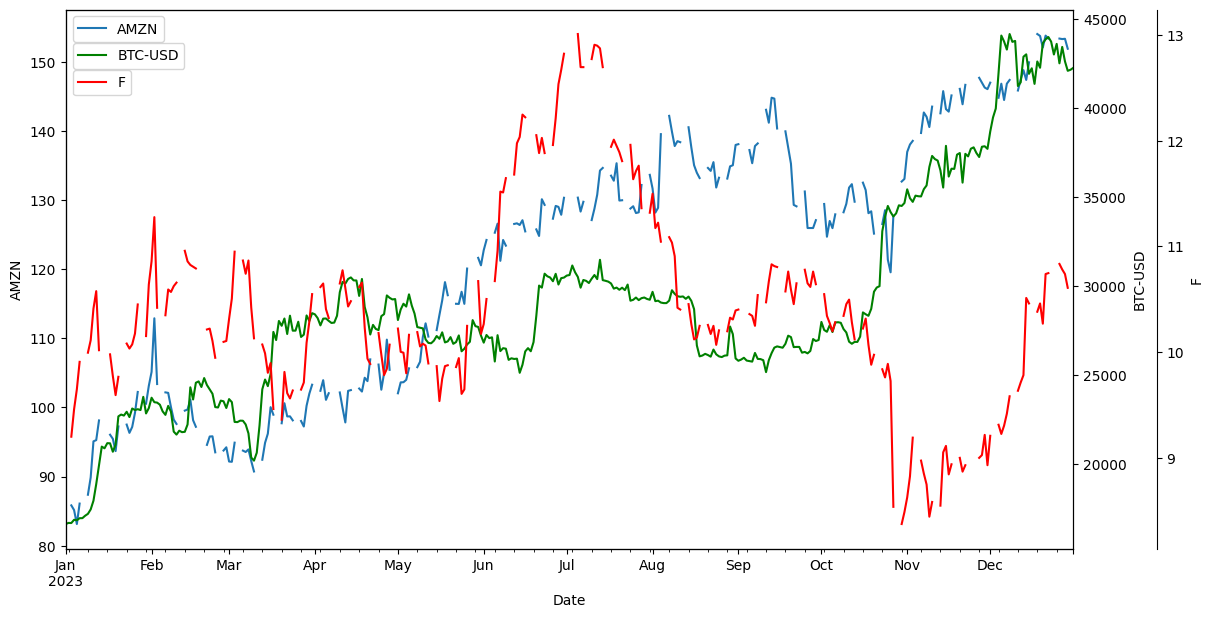
\includegraphics[width=\linewidth,height=0.6\textheight,keepaspectratio]{gfx/m2l1_notes_fig1_plot.png}
\par\smallskip{\small \textbf{Hình 1.1:} Giá AMZN, Bitcoin (BTC-USD) và Ford năm 2023 trên ba trục y khác nhau}
\end{figure}

Mã và biểu đồ trên minh họa cách chúng ta có thể dễ dàng truyền một phạm vi ngày vào phương thức vẽ biểu đồ để vẽ một tập con của dữ liệu. Nếu không có phạm vi ngày nào được cung cấp, theo mặc định, biểu đồ sẽ bao gồm toàn bộ tập dữ liệu. Đoạn mã này tạo ra một figure với ba biểu đồ con chia sẻ cùng một trục x (ngày) nhưng có các trục y khác nhau để vẽ giá của Amazon (AMZN), Bitcoin (BTC-USD) và Ford (F) cho năm 2023. Cách tiếp cận này cho phép chúng ta hình dung xu hướng giá của ba tài sản khác nhau với các thang đo khác nhau trên cùng một biểu đồ. Tuy nhiên, biểu đồ cũng minh họa lý do tại sao chỉ sử dụng giá không phải là lý tưởng để so sánh hai tài sản. Thang đo giá của Bitcoin so với một cổ phiếu giá thấp như Ford khiến việc so sánh hai cổ phiếu này trở nên rất khó khăn khi quyết định đầu tư vào cổ phiếu nào tốt hơn.

\section{Tính toán Lợi suất Đầu tư}

Nếu chúng ta đầu tư \textbf{\$1,000} vào mỗi tài sản này năm năm trước, hôm nay chúng ta sẽ có bao nhiêu tiền? Để trả lời câu hỏi này, trước tiên chúng ta cần xác định chúng ta có thể mua bao nhiêu cổ phiếu của mỗi loại với \textbf{\$1,000} vào đầu phạm vi ngày của chúng ta. Đối với mục đích của bài tập này, chúng ta sẽ sử dụng \textbf{01/08/2019} làm điểm bắt đầu vì i

Từ dữ liệu của chúng ta ở trên, chúng ta có thể thấy giá khởi điểm của AMZN, F và Bitcoin. Chúng ta cũng có thể lưu trữ giá trị của hàng đầu tiên cho mỗi mã trong các biến riêng lẻ, mà sau đó chúng ta có thể sử dụng cho các tính toán hoặc phân tích sâu hơn. Chúng ta sẽ thực hiện việc này trong đoạn mã sau. Chúng ta cũng cần chia \textbf{\$1,000} cho mỗi con số này để xem chúng ta sẽ có bao nhiêu cổ phiếu:

\begin{lstlisting}[language=Python,escapeinside={(*@}{@*)}]
# Truy (*@cập@*) (*@hàng@*) (*@đầu@*) (*@tiên@*) (*@của@*) DataFrame
first_row = df.iloc[0]

# (*@Gán@*) (*@các@*) (*@giá@*) (*@trị@*) (*@giá@*) cho (*@các@*) (*@biến@*)
amzn_price = first_row["AMZN"]
f_price = first_row["F"]
btc_price = first_row["BTC-USD"]

# In (*@các@*) (*@giá@*) (*@trị@*) (*@giá@*)
print("Purchase price of AMZN:", np.round(amzn_price, 3))
print("Purchase price of F:", np.round(f_price, 3))
print("Purchase price of BTC-USD:", np.round(btc_price, 3))
print(" - - - - - - - - - -")

# Chia $1,000 cho (*@mỗi@*) (*@giá@*) (*@trị@*) (*@giá@*) (*@để@*) (*@lấy@*) (*@số@*) (*@lượng@*) (*@cổ@*) (*@phiếu@*)
amzn_shares = 1000 / amzn_price
f_shares = 1000 / f_price
btc_shares = 1000 / btc_price

# In (*@số@*) (*@lượng@*) (*@cổ@*) (*@phiếu@*) cho (*@mỗi@*) (*@mã@*)
print("Number of shares of AMZN:", np.round(amzn_shares, 3))
print("Number of shares of F:", np.round(f_shares, 3))
print("Number of shares of BTC-USD:", np.round(btc_shares, 3))
\end{lstlisting}

\begin{lstlisting}[escapeinside={(*@}{@*)}]
Purchase price of AMZN: 92.766
Purchase price of F: 6.834
Purchase price of BTC-USD: 10399.669
 - - - - - - - - - -
Number of shares of AMZN: 10.78
Number of shares of F: 146.334
Number of shares of BTC-USD: 0.096
\end{lstlisting}

Đây là một hiện tượng tương đối gần đây khi các nhà môi giới bán lẻ cung cấp các cổ phiếu lẻ (fractional shares), nhưng điều này có xu hướng trở thành trường hợp ngày nay đối với hầu hết các nhà môi giới thường được sử dụng. Đối với bài tập này, chúng ta sẽ giả định rằng chúng ta có thể có các cổ phiếu lẻ.

Bây giờ, để xác định hôm nay chúng ta sẽ có bao nhiêu tiền, chúng ta xem xét ngày gần nhất trong tập dữ liệu của chúng ta (31/07/2024), lấy giá của từng tài sản và nhân số lượng cổ phiếu của chúng ta với con số này. Chúng ta có thể tìm thấy điều này bằng cách nhìn vào cuối tập dữ liệu của chúng ta trong việc sử dụng phương thức \emph{tail()}. Ngoài ra, chúng ta cũng có thể lập trình các tính toán giá trị tài sản:

\begin{lstlisting}[language=Python,escapeinside={(*@}{@*)}]
# (*@Lấy@*) (*@các@*) (*@giá@*) (*@trị@*) (*@ngày@*) (*@cuối@*) (*@cùng@*) (*@từ@*) df
last_row = df.iloc[-1]

# (*@Gán@*) (*@các@*) (*@giá@*) (*@trị@*) (*@giá@*) (*@của@*) (*@ngày@*) (*@kết@*) (*@thúc@*) cho (*@các@*) (*@biến@*)
amzn_price_end = last_row["AMZN"]
f_price_end = last_row["F"]
btc_price_end = last_row["BTC-USD"]

# In (*@giá@*) (*@ngày@*) (*@kết@*) (*@thúc@*)
print("End price of AMZN:", np.round(amzn_price_end, 3))
print("End price of F:", np.round(f_price_end, 3))
print("End price of BTC-USD:", np.round(btc_price_end, 3))
print(" - - - - - - - - - -")

# (*@Tính@*) (*@toán@*) (*@các@*) (*@giá@*) (*@trị@*) (*@ngày@*) (*@kết@*) (*@thúc@*) cho (*@mỗi@*) (*@mã@*)
amzn_value = amzn_price_end * amzn_shares  # (*@cần@*) (*@nhân@*) 20 (*@lần@*) do chia (*@tách@*) (*@cổ@*) (*@phiếu@*)
f_value = f_price_end * f_shares
btc_value = btc_price_end * btc_shares

# In (*@các@*) (*@giá@*) (*@trị@*) (*@ngày@*) (*@kết@*) (*@thúc@*)
print("Holding value of AMZN:", np.round(amzn_value, 3))
print("Holding value of F:", np.round(f_value, 3))
print("Holding value of BTC-USD:", np.round(btc_value, 3))
\end{lstlisting}

\begin{lstlisting}[escapeinside={(*@}{@*)}]
End price of AMZN: 186.98
End price of F: 9.786
End price of BTC-USD: 64619.25
 - - - - - - - - - -
Holding value of AMZN: 2015.609
Holding value of F: 1432.036
Holding value of BTC-USD: 6213.587
\end{lstlisting}

Khoản chi tiêu đầu tư là \$1000 cho mỗi mã. Bây giờ, dựa trên các kết quả tính toán ở trên, có vẻ như các khoản đầu tư của chúng ta đã hoạt động khác nhau:

\begin{itemize}
  \item AMZN: Khoản đầu tư Amazon của chúng ta đã tăng hơn gấp đôi, cho thấy một mức tăng đáng kể.
  \item F: Khoản đầu tư Ford của chúng ta cũng đã tăng trưởng, cho thấy một mức lợi suất khá tốt.
  \item BTC-USD: Khoản đầu tư Bitcoin của chúng ta đã tăng hơn sáu lần, cho thấy một khoản lợi nhuận đáng kể.
\end{itemize}
Tuy nhiên, điều quan trọng cần nhớ là đây chỉ là những giá trị cuối cùng và không kể toàn bộ câu chuyện. Để có bức tranh rõ ràng hơn về hiệu suất đầu tư, chúng ta cần xem xét:

\begin{itemize}
  \item Khung thời gian: Chúng ta cần biết khung thời gian của khoản đầu tư này để đánh giá lợi suất một cách chính xác. Những biến động ngắn hạn là bình thường, trong khi các xu hướng dài hạn cho thấy hiệu suất tổng thể tốt hơn.
  \item Các Yếu tố Bên ngoài: Độ biến động của thị trường, điều kiện kinh tế và tin tức cụ thể của công ty có thể tác động đáng kể đến giá cổ phiếu.
  \item Chiến lược Đầu tư: Các mục tiêu đầu tư cá nhân và khả năng chấp nhận rủi ro nên hướng dẫn các quyết định của bạn.
\end{itemize}
Các tài sản này tương đối dễ so sánh ở đây vì chúng ta bắt đầu với \$1,000 trong mỗi tài sản. Nếu chúng ta bắt đầu với các giá trị khác nhau, chúng ta sẽ cần tính toán lợi suất để có sự so sánh đồng nhất (apples-to-apples). Trong một bài học tương lai, chúng ta sẽ xem xét các lợi suất đơn giản và log, nhưng để thuận tiện, chúng ta sẽ sử dụng lợi suất đơn giản:

Công thức Lợi suất Đơn giản (Simple Returns Formula)

\[R_{simple} = \frac{p_{_1} - p_{_0}}{p_{_0}}\]

trong đó $p_{_1}$ = giá trị cuối, $p_{_0}$ = giá trị đầu

Điều này sẽ dễ dàng trong trường hợp của chúng ta vì \$1,000 là giá trị ban đầu trong cả ba tình huống.

\begin{lstlisting}[language=Python,escapeinside={(*@}{@*)}]
# (*@Tính@*) (*@toán@*) (*@lợi@*) (*@suất@*) (*@đơn@*) (*@giản@*)
amzn_return = (amzn_value - 1000) / 1000
f_return = (f_value - 1000) / 1000
btc_return = (btc_value - 1000) / 1000

# In (*@các@*) (*@lợi@*) (*@suất@*)
print("Simple return of AMZN:", np.round(amzn_return * 100, 3), "%")
print("Simple return of F:", np.round(f_return * 100, 3), "%")
print("Simple return of BTC-USD:", np.round(btc_return * 100, 3), "%")
\end{lstlisting}

\begin{lstlisting}[escapeinside={(*@}{@*)}]
Simple return of AMZN: 101.561 %
Simple return of F: 43.204 %
Simple return of BTC-USD: 521.359 %
\end{lstlisting}

Lợi suất của Bitcoin ở đây cao vượt trội so với hai tài sản còn lại. Bitcoin là một tài sản tương đối mới --- một số người thậm chí còn cho là rủi ro hơn --- so với hai tài sản kia. Rủi ro cao hơn đồng nghĩa với tiềm năng phần thưởng cao hơn, và cho đến nay, việc đầu tư vào Bitcoin đã mang lại kết quả hậu hĩnh.

\section{So sánh Cổ phiếu và Bitcoin với Trái phiếu}

Hãy giới thiệu thêm một loại tài sản nữa ở đây: trái phiếu. Như bạn nhớ từ lớp Thị trường Tài chính, trái phiếu không chỉ có hoàn trả tiền gốc, mà chúng còn trả một khoản phiếu giảm giá (coupon), thường là hàng năm hoặc hàng quý. Để đơn giản hóa mọi thứ, chúng ta sẽ sử dụng một quỹ hoán đổi danh mục (ETF), theo dõi các trái phiếu. ETF là quỹ Vanguard Long-Term Bond Index Fund ETF hoặc gọi tắt là BLV. Quỹ này dự định theo dõi hiệu suất của Chỉ số Bloomberg Barclays U.S. Long Government/Credit Float Adjusted Index. Chỉ số này bao gồm trái phiếu doanh nghiệp cấp đầu tư, chính phủ Hoa Kỳ và trái phiếu định danh bằng đô la quốc tế có kỳ hạn lớn hơn 10 năm. Ít nhất 80\% tổng tài sản của quỹ sẽ được đầu tư vào các trái phiếu được giữ trong chỉ số được đề cập ở trên (Vanguard).

Đoạn mã sau sẽ trích xuất dữ liệu BLV và kết hợp nó với DataFrame hiện tại của chúng ta, df.

\begin{lstlisting}[language=Python,escapeinside={(*@}{@*)}]
# (*@Để@*) (*@chuyển@*) (*@đổi@*) (*@giữa@*) (*@tải@*) (*@xuống@*) (*@dữ@*) (*@liệu@*) (*@trực@*) (*@tiếp@*) (*@và@*) (*@tải@*) (*@dữ@*) (*@liệu@*) (*@cục@*) (*@bộ,@*) 
# (*@bỏ@*) ghi (*@chú@*) (*@dòng@*) mong (*@muốn@*) (*@và@*) ghi (*@chú@*) (*@dòng@*) (*@còn@*) (*@lại.@*)
#df = df.join(yfin.download(["BLV"], start, end, auto_adjust = False)["Adj Close"].tz_localize('UTC'))
df = df.join(pd.read_csv('FD_M2_L1_stocks_data.csv', index_col='Date', parse_dates=True)\
             .loc[start:end].reindex(columns=["BLV"]).tz_localize('UTC'))
df
\end{lstlisting}

\begin{lstlisting}[escapeinside={(*@}{@*)}]
AMZN
F
BTC-USD
BLV


Date








2019-08-01 00:00:00+00:00
92.765999
6.833697
10,399.668945
74.656052


2019-08-02 00:00:00+00:00
91.162003
6.811677
10,518.174805
75.178711


2019-08-03 00:00:00+00:00
NaN
NaN
10,821.726562
NaN


2019-08-04 00:00:00+00:00
NaN
NaN
10,970.184570
NaN


2019-08-05 00:00:00+00:00
88.256500
6.774976
11,805.653320
75.822662


...
...
...
...
...


2024-07-27 00:00:00+00:00
NaN
NaN
67,813.335938
NaN


2024-07-28 00:00:00+00:00
NaN
NaN
68,255.867188
NaN


2024-07-29 00:00:00+00:00
183.199997
9.957947
66,819.914062
67.110588


2024-07-30 00:00:00+00:00
181.710007
9.804191
66,201.015625
67.251205


2024-07-31 00:00:00+00:00
186.979996
9.786100
64,619.250000
67.860443



1827 rows (*@$\times$@*) 4 columns
\end{lstlisting}

\subsection{Tính toán Lợi suất Log, Loại bỏ các Cột không sử dụng và Xóa Nulls}

Trước khi tính toán lợi suất, chúng ta cần loại bỏ các null cho các ngày cuối tuần.

\begin{lstlisting}[language=Python,escapeinside={(*@}{@*)}]
# (*@Để@*) (*@tính@*) (*@toán@*) (*@lợi@*) (*@suất@*) (*@của@*) (*@cổ@*) (*@phiếu,@*) (*@chúng@*) ta (*@cần@*) (*@loại@*) (*@bỏ@*) (*@các@*) (*@hàng@*) NA.
returns_stocks_BLV = df[['AMZN', 'F', 'BLV']].dropna().pct_change()

# Crypto (*@được@*) giao (*@dịch@*) 24/7
returns_BTC = df[['BTC-USD']].pct_change()

# (*@Chúng@*) ta (*@truyền@*) (broadcast) (*@chỉ@*) (*@mục@*) (*@của@*) crypto (*@vào@*) (*@các@*) (*@cổ@*) (*@phiếu@*) (*@để@*) (*@kết@*) (*@hợp@*) (*@các@*) (*@tập@*) (*@dữ@*) (*@liệu@*) 
# (*@có@*) NaN cho (*@các@*) (*@ngày@*) (*@cuối@*) (*@tuần@*) trong (*@các@*) (*@cột@*) (*@cổ@*) (*@phiếu@*) (*@và@*) BLV
returns_stocks = returns_stocks_BLV.reindex(returns_BTC.index)
returns = returns_BTC.join(returns_stocks_BLV, how = 'outer')[1:]
returns
\end{lstlisting}

\begin{lstlisting}[escapeinside={(*@}{@*)}]
BTC-USD
AMZN
F
BLV


Date








2019-08-02 00:00:00+00:00
0.011395
-0.017291
-0.003222
0.007001


2019-08-03 00:00:00+00:00
0.028860
NaN
NaN
NaN


2019-08-04 00:00:00+00:00
0.013719
NaN
NaN
NaN


2019-08-05 00:00:00+00:00
0.076158
-0.031872
-0.005388
0.008566


2019-08-06 00:00:00+00:00
-0.027740
0.012860
0.027086
0.006694


...
...
...
...
2024-07-27 00:00:00+00:00
-0.001454
NaN
NaN
NaN


2024-07-28 00:00:00+00:00
0.006526
NaN
NaN
NaN


2024-07-29 00:00:00+00:00
-0.021038
0.003836
-0.016086
0.003785


2024-07-30 00:00:00+00:00
-0.009262
-0.008133
-0.015441
0.002095


2024-07-31 00:00:00+00:00
-0.023893
0.029002
-0.001845
0.009059



1826 rows (*@$\times$@*) 4 columns
\end{lstlisting}

\subsection{Hiển thị Thống kê Tóm tắt cho Lợi suất}

\begin{lstlisting}[language=Python,escapeinside={(*@}{@*)}]
returns.describe()
\end{lstlisting}

\begin{lstlisting}[escapeinside={(*@}{@*)}]
BTC-USD
AMZN
F
BLV




count
1,826.000000
1,257.000000
1,257.000000
1,257.000000


mean
0.001579
0.000803
0.000671
-0.000034


std
0.033707
0.022175
0.027760
0.009179


min
-0.371695
-0.140494
-0.183614
-0.075169


25%
-0.013480
-0.011068
-0.013605
-0.005253


50%
0.000234
0.000643
0.000000
0.000572


75%
0.015996
0.012222
0.014212
0.005205


max
0.187465
0.135359
0.234414
0.049139
\end{lstlisting}

\subsection{Chuyển đổi Lợi suất Hàng ngày sang Hàng năm}

\begin{lstlisting}[language=Python,escapeinside={(*@}{@*)}]
(returns.describe()[["BTC-USD", "F"]])
\end{lstlisting}

\begin{lstlisting}[escapeinside={(*@}{@*)}]
BTC-USD
F




count
1,826.000000
1,257.000000


mean
0.001579
0.000671


std
0.033707
0.027760


min
-0.371695
-0.183614


25%
-0.013480
-0.013605


50%
0.000234
0.000000


75%
0.015996
0.014212


max
0.187465
0.234414
\end{lstlisting}

Vì chúng ta đang sử dụng lợi suất đơn giản, để chuẩn hóa chúng theo năm một cách chính xác, chúng ta sẽ sử dụng trung bình nhân (geometric mean):

\[ R_{\text{Geom\_Mean}} = \left( \prod_{i=1}^{N} \left( 1 + r_{i} \right) \right)^{\frac{1}{N}} - 1 \]

Sau đó, lợi suất hàng năm sẽ được tính bằng:

\[ R_{\text{Annaulized\_Returns}} = \left( R_{\text{Geom\_Mean}} + 1 \right)^{252 \text{ or } 365} - 1 \]

\begin{lstlisting}[language=Python,escapeinside={(*@}{@*)}]
# (*@Chuẩn@*) (*@hóa@*) BTC-USD theo (*@năm@*) (*@với@*) 365 (*@ngày@*) giao (*@dịch@*)
(np.prod(returns_BTC + 1, axis=0) ** (1/len(returns_BTC))) ** (365) - 1
\end{lstlisting}

\begin{lstlisting}[escapeinside={(*@}{@*)}]
BTC-USD   0.440439
dtype: float64
\end{lstlisting}

\begin{lstlisting}[language=Python,escapeinside={(*@}{@*)}]
# (*@Chuẩn@*) (*@hóa@*) (*@cổ@*) (*@phiếu@*) theo (*@năm@*) (*@với@*) 252 (*@ngày@*) giao (*@dịch@*)
(np.prod(returns_stocks_BLV + 1, axis=0) ** (1/len(returns_stocks_BLV))) ** (252) - 1
\end{lstlisting}

\begin{lstlisting}[escapeinside={(*@}{@*)}]
AMZN    0.150742
F       0.074584
BLV    -0.018936
dtype: float64
\end{lstlisting}

Chúng ta có thể chạy phân tích tương tự trên BLV giống như chúng ta đã làm trên các cổ phiếu ở trên để lấy tổng lợi suất đơn giản trong khoảng thời gian năm năm bằng cách sử dụng một phương pháp hơi khác. Lần này, chúng ta sẽ tính lợi suất đơn giản và sau đó chỉ nhân khoản đầu tư ban đầu 1,000 đô la với 1 + \texttt{returnRate}.

\begin{lstlisting}[language=Python,escapeinside={(*@}{@*)}]
# (*@Lấy@*) (*@giá@*) ban (*@đầu@*) (*@và@*) (*@giá@*) (*@cuối@*) (*@từ@*) df
blv_price = df.iloc[0]["BLV"]
blv_price_end = df.iloc[-1]["BLV"]

# (*@Tính@*) (*@lợi@*) (*@suất@*) (*@đơn@*) (*@giản@*)
blv_return_rate = (blv_price_end - blv_price) / blv_price
print("Simple return rate of BLV:", np.round(blv_return_rate * 100, 3), "%")

# (*@Tính@*) (*@tổng@*) (*@lợi@*) (*@suất@*) (*@đơn@*) (*@giản@*)
total_simple_return = 1000 * (1 + blv_return_rate)
print("Total simple return of BLV: $", np.round(total_simple_return, 3))
\end{lstlisting}

\begin{lstlisting}[escapeinside={(*@}{@*)}]
Simple return rate of BLV: -9.103 %
Total simple return of BLV: $ 908.974
\end{lstlisting}

Đầu ra này chỉ ra rằng khoản đầu tư vào BLV đã trải qua mức lợi suất đơn giản âm là -9.103\%. Điều này có nghĩa là chúng ta đã mất khoảng 9.1\% khoản đầu tư ban đầu của mình vào BLV.

Nếu chúng ta bắt đầu với 1.000 USD, sau năm năm, chúng ta sẽ thu về (1 - 9.103) * 1000 = 908.97 USD.

Đây là mức lợi suất thấp hơn nhiều so với những gì chúng ta sẽ nhận được với Ford, Amazon hoặc Bitcoin. Điều này được dự đoán phần lớn vì trái phiếu trả coupon (lãi suất) hàng quý/hàng năm cùng với việc hoàn trả tiền gốc. Vì lý do này, trái phiếu (đặc biệt là trái phiếu chính phủ) được coi là tài sản an toàn hơn cổ phiếu hoặc tiền điện tử. Một điều chính cần xem xét là nếu một công ty phá sản, bạn có thể không nhận lại được tiền gốc trong một trái phiếu. Điều đó nói lên rằng, điều tương tự cũng áp dụng cho cổ phiếu. Người nắm giữ trái phiếu cũng có rủi ro tín dụng thấp hơn so với người nắm giữ cổ phiếu: nếu bạn sở hữu một trái phiếu của Ford và bạn của bạn sở hữu cổ phiếu Ford, nhưng Ford tuyên bố phá sản vào ngày mai, người nắm giữ trái phiếu sẽ được thanh toán trước trong các thủ tục phá sản và chủ sở hữu vốn cổ phần sẽ chỉ nhận được những gì còn sót lại, làm cho trái phiếu trở thành một khoản đầu tư an toàn hơn.

Nhược điểm của điều này là rất khó để đạt được mức tổng lợi suất mà một cổ phiếu hoặc tiền điện tử có thể đạt được với một trái phiếu. Có một sự đánh đổi giữa rủi ro và phần thưởng (risk-reward tradeoff). Hãy nghĩ lại về bài đọc trong bài học này một chút. Những gì chúng ta vừa thảo luận ở đây được đề cập trong bài đọc so sánh một khoản đầu tư có phương sai cao (high-variance) với một khoản đầu tư có phương sai thấp (low-variance). Bạn chọn gì hoàn toàn phụ thuộc vào sở thích rủi ro của bạn. Luôn xem xét sự đánh đổi giữa rủi ro và phần thưởng.

Dưới đây là một số điểm cần xem xét:

\begin{itemize}
  \item \textbf{Thời gian Đầu tư (Time Horizon):} Lợi suất đơn giản không tính đến khung thời gian đầu tư. Những khoản lỗ ngắn hạn không phải là bất thường, và điều quan trọng là phải đánh giá các khoản đầu tư trong một thời gian dài hơn để có được bức tranh chính xác hơn về hiệu suất của chúng.
  \item \textbf{Đo lường chuẩn (Benchmarking):} So sánh lợi suất của BLV với một điểm chuẩn (benchmark) có liên quan, chẳng hạn như chỉ số thị trường rộng lớn như S\&P 500, để đánh giá hiệu suất tương đối của nó.
  \item \textbf{Chiến lược Đầu tư:} Xem xét các mục tiêu đầu tư tổng thể và khả năng chịu rủi ro của bạn khi đánh giá hiệu suất của BLV.
\end{itemize}
Hãy nhớ rằng lợi suất đơn giản chỉ là một cách để đo lường hiệu suất đầu tư. Để phân tích toàn diện hơn, hãy xem xét các yếu tố như cổ tức, thuế, tính thanh khoản, quy định, rủi ro tín dụng, biến động và giá trị thời gian của tiền.

\section{Giá trị Tương lai của một Khoản đầu tư}

S\&P 500 bao gồm 500 công ty vốn hóa lớn. Chỉ số này tính toán trọng số theo vốn hóa thị trường. Trọng số này khác với trọng số trong Chỉ số Trung bình Công nghiệp Dow Jones, được tính trọng số theo giá. Các công ty tạo nên chỉ số này được lựa chọn bởi một ủy ban, nhưng các công ty phải đáp ứng các tiêu chí cụ thể trước khi được đưa vào (Standard \& Poor's):

\begin{itemize}
  \item Vốn hóa thị trường phải lớn hơn hoặc bằng 18 tỷ USD.
  \item Giá trị đô la hàng năm được giao dịch trên vốn hóa thị trường được điều chỉnh theo khối lượng tự do chuyển nhượng lớn hơn 1.0.
  \item Khối lượng giao dịch tối thiểu hàng tháng là 250.000 cổ phiếu trong mỗi sáu tháng tính đến ngày đánh giá.
  \item Công ty phải được niêm yết công khai trên Sở Giao dịch Chứng khoán New York (NYSE), bao gồm NYSE Arca hoặc NYSE American, hoặc NASDAQ (NASDAQ Global Select Market, NASDAQ Select Market hoặc NASDAQ Capital Market).
  \item Công ty phải từ Hoa Kỳ.
  \item Các chứng khoán không đủ điều kiện để đưa vào chỉ số là các công ty hợp danh hữu hạn, công ty hợp danh hữu hạn chính và các đơn vị ủy thác đầu tư của họ, các vấn đề của OTC Bulletin Board, quỹ đóng, quỹ hoán đổi danh mục, trái phiếu hoán đổi danh mục, ủy thác tiền bản quyền, cổ phiếu theo dõi, cổ phiếu ưu đãi, ủy thác đơn vị, chứng quyền cổ phần, trái phiếu chuyển đổi, ủy thác đầu tư, biên lai lưu ký Mỹ và cổ phiếu lưu ký Mỹ.
  \item Kể từ năm 2017, các công ty có cấu trúc cổ phiếu hai loại, như Standard \& Poor's, không được thêm vào chỉ số.
\end{itemize}
Điều này sẽ được sử dụng như là đại diện (proxy) của chúng ta cho các cổ phiếu vốn hóa lớn.

Russell 2000 là một chỉ số chứa 2.000 công ty vốn hóa nhỏ và thường xuyên được sử dụng như một điểm chuẩn bởi các quỹ tương hỗ vốn hóa nhỏ cho mục đích so sánh. Russell 2000 được cấu trúc để cung cấp một thước đo cho các cổ phiếu vốn hóa nhỏ. Nó được tái cấu trúc hàng năm để đảm bảo các công ty từ năm trước không trở nên quá lớn và làm biến dạng các đặc điểm của vốn hóa nhỏ (Maginn 118).

Chỉ số Russell 2000 sẽ được sử dụng như là đại diện của chúng ta cho các công ty vốn hóa nhỏ.

Một cách để so sánh hai cơ hội đầu tư là xác định giá trị tương lai của một khoản đầu tư. Luôn có những rủi ro và nhiều giả định cần được đưa ra khi xác định giá trị tương lai, đặc biệt là đối với một khoản đầu tư rủi ro như một cổ phiếu. Chúng ta sẽ bắt đầu bằng cách sử dụng lợi suất trung bình hàng ngày của mỗi chỉ số để xác định lợi suất kỳ vọng. Đây là một cách suy nghĩ đơn giản vì không thể nói rằng 10 năm tới sẽ giống hệt như 10 năm qua, nhưng nó là một điểm khởi đầu khi so sánh các khoản đầu tư. Chúng ta sẽ đi sâu hơn vào các số liệu so sánh nâng cao hơn khi khóa học tiếp diễn.

\textbf{Công thức tính lãi kép là:}

\[FV = PV (1+i)^n\]

trong đó

$FV$ = Giá trị tương lai $PV$ = Giá trị hiện tại $i$ = Lãi suất định kỳ $n$ = Số kỳ

\subsection{Lấy dữ liệu giá hàng ngày trong 5 năm cho S\&P 500 và Russell 2000}

Chúng ta sẽ đi sâu hơn vào các loại tài sản cổ phiếu cụ thể và so sánh chúng như những khoản đầu tư tiềm năng. Chúng ta sẽ bắt đầu bằng cách so sánh cổ phiếu vốn hóa lớn với cổ phiếu vốn hóa nhỏ bằng cách sử dụng S\&P 500 và Chỉ số Russell 2000.

Xuyên suốt bài học này, chúng ta sẽ xây dựng hướng tới một hàm ở đây nhận vào một phạm vi ngày và so sánh hai chuỗi lợi suất.

\begin{lstlisting}[language=Python,escapeinside={(*@}{@*)}]
# (*@Ngày@*) (*@tháng@*)
start = datetime.date(2019, 8, 1)
end = datetime.date(2024, 8, 1)

# (*@Để@*) (*@chuyển@*) (*@đổi@*) (*@giữa@*) (*@việc@*) (*@tải@*) (*@dữ@*) (*@liệu@*) (*@trực@*) (*@tiếp@*) (*@và@*) (*@tải@*) (*@dữ@*) (*@liệu@*) (*@cục@*) (*@bộ,@*) 
# (*@bỏ@*) ghi (*@chú@*) (*@dòng@*) mong (*@muốn@*) (*@và@*) ghi (*@chú@*) (*@dòng@*) (*@còn@*) (*@lại.@*)
#prices = yfin.download(["^GSPC", "^RUT"], start, end, auto_adjust = False)["Adj Close"]
prices = pd.read_csv('FD_M2_L1_stocks_data.csv', index_col='Date', parse_dates=True)\
                        .loc[start:end].reindex(columns=["^GSPC", "^RUT"])

# (*@Đổi@*) (*@tên@*) (*@cột@*) (*@để@*) (*@làm@*) cho (*@tên@*) (*@trực@*) quan (*@hơn@*)
prices = prices.rename(columns={"^GSPC": "SP500", "^RUT": "Russell2000"})

# (*@Lấy@*) (*@thống@*) (*@kê@*) (*@của@*) (*@tập@*) (*@dữ@*) (*@liệu@*)
prices.describe()
\end{lstlisting}

\begin{lstlisting}[escapeinside={(*@}{@*)}]
SP500
Russell2000




count
1,258.000000
1,258.000000


mean
4,028.833253
1,865.957234


std
685.682781
284.232353


min
2,237.399902
991.159973


25%
3,502.235046
1,674.337524


50%
4,110.745117
1,873.654968


75%
4,468.547485
2,067.780090


max
5,667.200195
2,442.739990
\end{lstlisting}

\begin{lstlisting}[language=Python,escapeinside={(*@}{@*)}]
# (*@Hiển@*) (*@thị@*) 5 (*@hàng@*) (*@đầu@*) (*@tiên@*)
prices.head()
\end{lstlisting}

\begin{lstlisting}[escapeinside={(*@}{@*)}]
SP500
Russell2000


Date






2019-08-01
2,953.560059
1,550.760010


2019-08-02
2,932.050049
1,533.660034


2019-08-03
NaN
NaN


2019-08-04
NaN
NaN


2019-08-05
2,844.739990
1,487.410034
\end{lstlisting}

Một lần nữa, chúng ta có thể thấy các tập dữ liệu này có các điểm bắt đầu khác nhau, vì vậy cách duy nhất chúng ta có thể thực hiện so sánh công bằng là so sánh lợi suất.

\subsection{Tính toán Lợi suất Log, Xóa Các Cột Không Sử Dụng và Loại bỏ Null}

Ở đây chúng ta có các giá trị null cho các ngày cuối tuần vì S\&P 500 và Chỉ số Russell 2000 đều là các chỉ số chứng khoán. Đoạn mã sau loại bỏ các giá trị null bằng phương thức \texttt{.df.dropna()} và tính toán lợi suất log của các tài sản tài chính này:

\begin{lstlisting}[language=Python,escapeinside={(*@}{@*)}]
# (*@Tính@*) (*@toán@*) (*@lợi@*) (*@suất@*) log
prices = prices.dropna()
df = np.log(prices) - np.log(prices.shift(1))
df = df.iloc[1:, 0:]
df.head()
\end{lstlisting}

\begin{lstlisting}[escapeinside={(*@}{@*)}]
SP500
Russell2000


Date






2019-08-02
-0.007309
-0.011088


2019-08-05
-0.030230
-0.030621


2019-08-06
0.012933
0.009821


2019-08-07
0.000767
-0.000932


2019-08-08
0.018588
0.020734
\end{lstlisting}

Lợi suất log thường được ưa thích hơn lợi suất đơn giản trong phân tích tài chính vì một số lý do:

\begin{itemize}
  \item Tính cộng dồn theo thời gian: Lợi suất log có thể dễ dàng được cộng lại qua thời gian để tính toán lợi suất tích lũy trong các khoảng thời gian dài hơn.
  \item Tính chuẩn: Lợi suất log có xu hướng phân phối chuẩn hơn so với lợi suất đơn giản, đây là một đặc tính mong muốn cho việc lập mô hình thống kê.
  \item Tính đối xứng: Lợi suất log cung cấp tính đối xứng tốt hơn lợi suất đơn giản, đặc biệt đối với những thay đổi nhỏ hơn, điều này làm cho chúng phù hợp hơn với một số loại phân tích tài chính.
\end{itemize}
Bằng cách tính toán lợi suất log, bạn có thể thực hiện phân tích và lập mô hình tài chính tinh vi hơn.

\subsection{Tính toán Giá trị Tương lai của Mỗi Chỉ số}

Trong đoạn mã sau, chúng ta tính toán lợi suất trung bình hàng năm cho mỗi chỉ số bằng cách sử dụng giá trị trung bình của lợi suất hàng ngày nhân với 252 (số ngày giao dịch mỗi năm). Sau đó, chúng ta sử dụng các lợi suất trung bình này để tính toán giá trị tương lai.

\begin{lstlisting}[language=Python,escapeinside={(*@}{@*)}]
# (*@Tính@*) (*@toán@*) (*@lợi@*) (*@suất@*) trung (*@bình@*) (*@hàng@*) (*@năm@*) trong 5 (*@năm@*) qua
avg_returns = df.mean() * 252

# (*@Tính@*) (*@toán@*) (*@giá@*) (*@trị@*) (*@tương@*) lai cho (*@mỗi@*) (*@chỉ@*) (*@số@*)
future_value_sp500 = 1000 * np.exp(avg_returns["SP500"] * 5)
future_value_russell2000 = 1000 * np.exp(avg_returns["Russell2000"] * 5)

print("Future Value of SP500:", future_value_sp500)
print("Future Value of Russell2000:", future_value_russell2000)
\end{lstlisting}

\begin{lstlisting}[escapeinside={(*@}{@*)}]
Future Value of SP500: 1872.5041981875975
Future Value of Russell2000: 1455.0892174400194
\end{lstlisting}

Hãy nhớ rằng hiệu suất trong quá khứ không phải là chỉ báo cho kết quả trong tương lai. Sử dụng lợi suất trung bình của 5 năm qua chỉ là một cách tiếp cận, và bạn nên xem xét các yếu tố khác và rủi ro tiềm ẩn khi đưa ra quyết định đầu tư.

Trong trường hợp cụ thể của chúng ta ở trên, vì chúng ta đang tính toán giá trị tương lai trong khoảng thời gian 5 năm, việc sử dụng lợi suất trung bình hàng năm có khả năng phù hợp và hiệu quả hơn. Tuy nhiên, nếu chúng ta đang phân tích những biến động ngắn hạn hoặc rủi ro của các chỉ số, lợi suất hàng ngày sẽ cung cấp nhiều thông tin hơn.

Việc tốt hơn nên tính toán lợi suất trung bình hàng ngày hay lợi suất trung bình hàng năm phụ thuộc vào bối cảnh và cách chúng ta dự định sử dụng kết quả. Dưới đây là sự phân tích chi tiết về các cân nhắc:

\begin{itemize}
  \item Khả năng so sánh: Nếu chúng ta muốn so sánh lợi suất của các tài sản hoặc khoản đầu tư khác nhau với các khung thời gian khác nhau, lợi suất hàng năm thường hữu ích hơn. Lợi suất hàng ngày có thể gây hiểu nhầm nếu các kỳ đầu tư không giống nhau.
  \item Tính toán Giá trị Tương lai: Nếu chúng ta đang đặc biệt tính toán các giá trị tương lai, việc sử dụng trực tiếp lợi suất trung bình hàng năm trong công thức sẽ đơn giản hơn và tránh được các bước bổ sung.
  \item Phân tích Biến động: Nếu chúng ta quan tâm đến việc phân tích sự biến động hoặc rủi ro của một khoản đầu tư, lợi suất hàng ngày có thể phù hợp hơn vì chúng cung cấp dữ liệu chi tiết hơn.
\end{itemize}
Viết lại đoạn mã trước bằng cách sử dụng lợi suất hàng ngày như sau:

\begin{lstlisting}[language=Python,escapeinside={(*@}{@*)}]
# (*@Tính@*) (*@toán@*) (*@lợi@*) (*@suất@*) trung (*@bình@*) (*@hàng@*) (*@ngày@*) trong 5 (*@năm@*) qua
avg_daily_returns = df.mean()

# (*@Tính@*) (*@toán@*) (*@giá@*) (*@trị@*) (*@tương@*) lai cho (*@mỗi@*) (*@chỉ@*) (*@số@*) (*@(sử@*) (*@dụng@*) (*@lợi@*) (*@suất@*) (*@hàng@*) (*@ngày@*) (*@và@*) 5 (*@năm)@*)
num_days = 252 * 5  # (*@Số@*) (*@ngày@*) giao (*@dịch@*) trong 5 (*@năm@*)
future_value_sp500 = 1000 * np.exp(avg_daily_returns["SP500"] * num_days)
future_value_russell2000 = 1000 * np.exp(avg_daily_returns["Russell2000"] * num_days)

print("Future Value of SP500:", future_value_sp500)
print("Future Value of Russell2000:", future_value_russell2000)
\end{lstlisting}

\begin{lstlisting}[escapeinside={(*@}{@*)}]
Future Value of SP500: 1872.5041981875975
Future Value of Russell2000: 1455.0892174400194
\end{lstlisting}

Cách tiếp cận này sử dụng lợi suất hàng ngày thay vì lợi suất hàng năm để tính toán giá trị tương lai. Hãy nhớ rằng điều này giả định việc tính lãi kép liên tục, có thể không hoàn toàn chính xác đối với các khoản đầu tư trong thế giới thực.

Đầu ra cho thấy giá trị tương lai của một khoản đầu tư ban đầu 1,000 đô la vào cả hai chỉ số S\&P 500 và Russell 2000 sau 5 năm, dựa trên lợi suất trung bình hàng ngày của chúng.

\begin{itemize}
  \item S\&P500: Giá trị tương lai xấp xỉ 1.872.50 đô la.
  \item Russell2000: Giá trị tương lai xấp xỉ 1.455.09 đô la.
\end{itemize}
Mặc dù giá trị tương lai rất quan trọng khi so sánh các khoản đầu tư, chúng ta cũng cần phải quan tâm đến mức độ biến động của các cơ hội đầu tư này. Trong phần tiếp theo, chúng ta sẽ thảo luận về ba số liệu biến động khác nhau cùng với cách lập trình chúng trong Python.

\section{Các Cơ hội Đầu tư: Sự Biến động}

\subsection{Biến động Giá: Cao-Thấp}

Chúng ta sẽ sử dụng lại DataFrame \texttt{prices} để chỉ ra một số cách đơn giản nhằm so sánh sự biến động của một số khoản đầu tư nhất định. Phương pháp đầu tiên là so sánh mức cao và mức thấp của chỉ số. Đối với điều này, chúng ta sử dụng các phương thức \texttt{max()} và \texttt{min()} để lấy mức cao và mức thấp trong khoảng thời gian của DataFrame theo cột. Từ đây, chúng ta có thể trừ chúng cho nhau để có ý tưởng về sự biến động tiềm năng của mỗi khoản đầu tư.

\begin{lstlisting}[language=Python,escapeinside={(*@}{@*)}]
prices.max()
\end{lstlisting}

\begin{lstlisting}[escapeinside={(*@}{@*)}]
SP500         5,667.200195
Russell2000   2,442.739990
dtype: float64
\end{lstlisting}

\begin{lstlisting}[language=Python,escapeinside={(*@}{@*)}]
prices.min()
\end{lstlisting}

\begin{lstlisting}[escapeinside={(*@}{@*)}]
SP500         2,237.399902
Russell2000     991.159973
dtype: float64
\end{lstlisting}

\begin{lstlisting}[language=Python,escapeinside={(*@}{@*)}]
prices.max() - prices.min()
\end{lstlisting}

\begin{lstlisting}[escapeinside={(*@}{@*)}]
SP500         3,429.800293
Russell2000   1,451.580017
dtype: float64
\end{lstlisting}

Mặc dù một số người có thể thấy điều này hữu ích, nhưng chúng ta chắc chắn cần cải thiện số liệu này để làm cho nó hữu ích hơn khi so sánh các khoản đầu tư khác nhau. Bạn nghĩ chúng ta có thể làm điều này như thế nào? Hãy thử hai ý tưởng.

Ý tưởng đầu tiên là thay đổi một chút khung thời gian. Ở trên, chúng ta đang xem xét dữ liệu 5 năm qua. Có lẽ sẽ hữu ích hơn khi phân tích dữ liệu gần đây hơn. Đối với điều này, chúng ta sẽ xem xét cùng một số liệu trong năm qua:

\begin{lstlisting}[language=Python,escapeinside={(*@}{@*)}]
# (*@Cắt@*) ra (*@năm@*) (*@ngoái@*) (*@từ@*) (*@dữ@*) (*@liệu@*) (*@giá@*)
end = pd.Timestamp(end).tz_localize(None)  # (*@Xóa@*) (*@thông@*) tin (*@múi@*) (*@giờ@*)

currYear = prices.loc[
    pd.Timestamp(end - datetime.timedelta(365)) : end
]

# (*@Tính@*) (*@sự@*) (*@khác@*) (*@biệt@*) (*@giữa@*) (*@các@*) (*@giá@*) (*@trị@*) (*@tối@*) (*@đa@*) (*@và@*) (*@tối@*) (*@thiểu@*) trong currYear
currYear.max() - currYear.min()
\end{lstlisting}

\begin{lstlisting}[escapeinside={(*@}{@*)}]
SP500         1,549.830078
Russell2000     626.729980
dtype: float64
\end{lstlisting}

Ngay cả khi so sánh dữ liệu trong 365 ngày qua, có vẻ khó để thực hiện một sự so sánh hai tập dữ liệu này vì chúng có các điểm bắt đầu khác nhau. Một sự điều chỉnh cuối cùng cho số liệu biến động này có thể là chuẩn hóa nó bằng cách chia cho mức giá hiện tại của chỉ số:

\begin{lstlisting}[language=Python,escapeinside={(*@}{@*)}]
(currYear.max() - currYear.min()) / prices.iloc[-1]
\end{lstlisting}

\begin{lstlisting}[escapeinside={(*@}{@*)}]
SP500         0.280649
Russell2000   0.277993
dtype: float64
\end{lstlisting}

Sự biến động là một thước đo của sự phân tán hoặc dao động của các mức lợi suất. Sự biến động cao hơn chỉ ra những sự thay đổi giá lớn hơn và rủi ro có khả năng cao hơn. Bây giờ chúng ta đã có dữ liệu được chuẩn hóa bằng mức giá hiện tại, số liệu cao/thấp này thực sự cho thấy rằng chúng ta có các mức biến động hàng ngày tương tự ở cả hai chỉ số, với S\&P 500 biến động hơn một chút so với Russell 2000.

\textbf{Lưu ý Quan trọng:}

\begin{itemize}
  \item Những giá trị này được dựa trên dữ liệu lịch sử và có thể không phản ánh sự biến động trong tương lai.
  \item Sự biến động có thể được tính toán bằng cách sử dụng các phương pháp và các khung thời gian khác nhau. Hãy đảm bảo bạn hiểu tính toán cụ thể được sử dụng để diễn giải các kết quả một cách chính xác.
  \item Việc hiểu sự biến động là rất quan trọng để đánh giá rủi ro đầu tư và đưa ra các quyết định sáng suốt.
\end{itemize}
\subsection{Trung bình trượt (Moving Averages)}

Chúng ta sẽ tạo một số liệu biến động so sánh giá của mỗi ngày với trung bình trượt. Các mức trung bình 50 ngày và 200 ngày thường được sử dụng khi so sánh các khoản đầu tư. Đối với số liệu của chúng ta, chúng ta sẽ sử dụng mức trung bình 50 ngày. Đây là một ví dụ về cách chúng ta có thể vẽ biểu đồ của S\&P 500 cùng với trung bình trượt 50 ngày của nó:

\begin{lstlisting}[language=Python,escapeinside={(*@}{@*)}]
# (*@Tính@*) trung (*@bình@*) (*@trượt@*) 50 (*@ngày@*) (*@của@*) (*@cột@*) "SP500"
prices["SP500 50 day_rolling_avg"] = prices.SP500.rolling(50).mean()

# (*@thiết@*) (*@lập@*) (*@kích@*) (*@thước@*) (*@hình@*) (*@vẽ@*) (*@và@*) (*@vẽ@*) (*@một@*) (*@biểu@*) (*@đồ@*) (*@chuỗi@*) (*@thời@*) gian (*@đơn@*) (*@giản@*) (*@bằng@*) (*@cách@*) (*@sử@*) (*@dụng@*) seaborn.lineplot()
plt.figure(figsize=(13, 7))
sns.lineplot(x="Date", y="SP500", data=prices, label="Daily S&P 500 Prices")

# (*@vẽ@*) trung (*@bình@*) (*@trượt@*)
sns.lineplot(x="Date", y="SP500 50 day_rolling_avg", data=prices, label="Rollingavg", linewidth=2)
plt.show()
\end{lstlisting}

\begin{figure}[H]
\centering
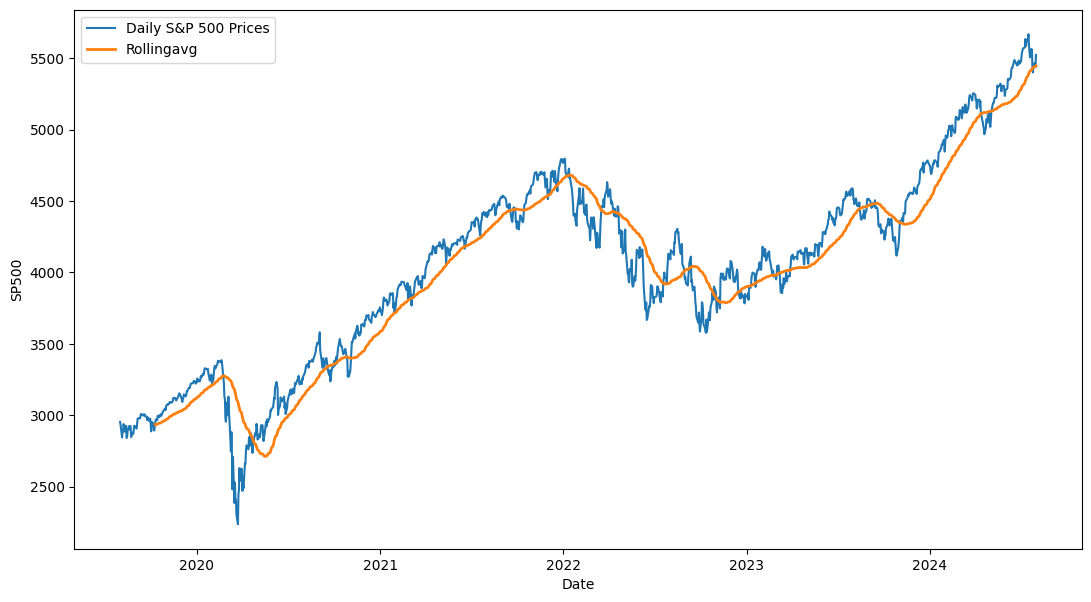
\includegraphics[width=\linewidth,height=0.6\textheight,keepaspectratio]{gfx/m2l1_notes_fig2_plot.png}
\par\smallskip{\small \textbf{Hình 1.2:} Giá S\&P 500 kèm đường trung bình trượt 50 ngày}
\end{figure}

Trực quan hóa này giúp làm phẳng các dao động ngắn hạn trong giá hàng ngày và làm nổi bật xu hướng dài hạn hơn của S\&P 500. Trung bình trượt cung cấp một bức tranh rõ ràng hơn về hướng đi tổng thể của thị trường.

\subsection{Các Khoảng cách Trượt}

Chúng ta có thể tạo một số liệu biến động ở đây bằng cách sử dụng trung bình trượt này. Hãy tưởng tượng chúng ta đang lấy khoảng cách giữa đường trung bình trượt và mỗi điểm dữ liệu từ biểu đồ S\&P 500. Chúng ta có thể sử dụng điều này như một đại diện (proxy) cho sự biến động. Chúng ta cũng sẽ muốn xử lý các sự khác biệt âm giống như các sự khác biệt dương; nếu không, chúng có thể triệt tiêu lẫn nhau. Do đó, chúng ta sẽ sử dụng giá trị tuyệt đối của mỗi điểm. Chúng ta sẽ chia các sự khác biệt này cho các mức giá để chuẩn hóa các giá trị này, và cuối cùng, chúng ta sẽ lấy trung bình của các giá trị đó. Điều này có thể được lập trình bằng Python với dòng mã đơn giản này:

\begin{lstlisting}[language=Python,escapeinside={(*@}{@*)}]
((abs(prices - prices.rolling(50).mean())) / prices).mean()
\end{lstlisting}

\begin{lstlisting}[escapeinside={(*@}{@*)}]
SP500                      0.037068
Russell2000                0.048725
SP500 50 day_rolling_avg   0.028209
dtype: float64
\end{lstlisting}

Kết quả của tính toán này cung cấp một thước đo về việc trung bình các mức giá hàng ngày lệch bao nhiêu so với trung bình trượt 50 ngày của chúng, được thể hiện dưới dạng một phần trăm. Điều này có thể là một chỉ báo hữu ích về sự biến động hoặc sự ổn định của tài sản. Các giá trị cao hơn đề xuất các dao động lớn hơn xung quanh trung bình trượt, trong khi các giá trị thấp hơn chỉ ra các mức giá ổn định hơn.

Đây là một số liệu khác biệt so với số liệu cao/thấp mà chúng ta đã tính toán trước đó, và nó cho thấy độ lệch trung bình cho Russell 2000 là biến động hơn khi so sánh với S\&P 500. Và bản thân trung bình trượt (SP500 50 day\_rolling\_avg) có một độ lệch trung bình là 2,82\%. Điều này là như được mong đợi vì trung bình trượt thì mượt hơn các mức giá hàng ngày.

Các giá trị này có thể hữu ích để hiểu sự biến động tương đối của các tài sản khác nhau và mức độ mà các giá hàng ngày có xu hướng đi lệch khỏi các xu hướng dài hạn hơn của chúng.

\subsection{Biến động Giá: Các Độ lệch chuẩn}

Độ lệch chuẩn có khả năng là số liệu biến động phổ biến nhất được sử dụng khi xem xét một cơ hội đầu tư. Nó đơn giản như việc gọi phương thức \texttt{std()} trên một DataFrame.

\begin{lstlisting}[language=Python,escapeinside={(*@}{@*)}]
prices.std()
\end{lstlisting}

\begin{lstlisting}[escapeinside={(*@}{@*)}]
SP500                      685.682781
Russell2000                284.232353
SP500 50 day_rolling_avg   635.644388
dtype: float64
\end{lstlisting}

Như đã đề cập trước đó, việc gọi phương thức này trên các mức giá không trực quan như việc gọi phương thức này trên các mức lợi suất vì các mức giá bắt đầu ở các điểm khác nhau. Để có một so sánh tốt hơn, chúng ta sẽ gọi phương thức \texttt{std()} này trên các mức lợi suất hàng ngày của 5 năm qua:

\begin{lstlisting}[language=Python,escapeinside={(*@}{@*)}]
df.std()
\end{lstlisting}

\begin{lstlisting}[escapeinside={(*@}{@*)}]
SP500         0.013458
Russell2000   0.017503
dtype: float64
\end{lstlisting}

Ở đây một lần nữa, Russell 2000 có một độ lệch chuẩn cao hơn một chút so với S\&P 500, đề xuất rằng nó đã biến động hơn trong 5 năm qua.

\subsection{Viết một Hàm So sánh Biến động trong Python}

Để kết nối tất cả lại với nhau, chúng ta sẽ lấy ba số liệu biến động mà chúng ta đã sử dụng cho đến thời điểm này, cùng với lợi suất hàng ngày trung bình, và viết một hàm, trong đó lấy:

\begin{itemize}
  \item \texttt{startTime} - định dạng \texttt{dateTime} 
  \item \texttt{endTime} - định dạng \texttt{dateTime} 
  \item \texttt{tickers} - một từ điển của các giá trị trong đó khóa là mã yahoo và giá trị là tên hiển thị tức là \{``\textasciicircum{}GSPC'': ``SP500'', ``\textasciicircum{}RUT'': ``Russell2000''\}
\end{itemize}
Bằng cách viết một hàm như thế này, nó cho phép nghiên cứu của chúng ta có thể được tái tạo và áp dụng cho nhiều tham số khác nhau. Trong trường hợp của chúng ta, nó sẽ là một phạm vi ngày và từ điển của các mã. Nếu bạn đang viết một ứng dụng nghiêm túc, bạn sẽ cần phải có nhiều xử lý lỗi trong hàm này, chẳng hạn như đảm bảo rằng các tham số được truyền vào thuộc đúng kiểu dữ liệu. Trong trường hợp của chúng ta, chúng ta sẽ giả định các kiểu dữ liệu của các tham số là chính xác và phạm vi ngày thì dài hơn 365 ngày.

\begin{lstlisting}[language=Python,escapeinside={(*@}{@*)}]
def investCompare(startTime, endTime, tickers):
    # (*@lấy@*) (*@dữ@*) (*@liệu@*) (*@giá@*) (*@từ@*) yahoo -- (list(tickers.keys())) = ['^GSPC','^RUT']
    startTime = pd.Timestamp(startTime).tz_localize('UTC')
    endTime = pd.Timestamp(endTime).tz_localize('UTC')
    
    # (*@Bỏ@*) (*@bình@*) (*@luận/bình@*) (*@luận@*) (*@dòng@*) (*@phù@*) (*@hợp@*) (*@để@*) (*@Tải@*) (*@xuống@*) (*@dữ@*) (*@liệu@*) (*@trực@*) (*@tiếp@*) (*@HOẶC@*) (*@tải@*) (*@dữ@*) (*@liệu@*) (*@từ@*) file (*@cục@*) (*@bộ@*)
    #prices = yfin.download(list(tickers.keys()), startTime, endTime, auto_adjust = False)["Adj Close"]
    prices = pd.read_csv('FD_M2_L1_stocks_data.csv', index_col='Date', parse_dates=True)\
                        .tz_localize('UTC').loc[startTime:endTime].reindex(columns=list(tickers.keys()))
    prices = prices.rename(columns=tickers)
    
    # (*@Tính@*) (*@toán@*) (*@lợi@*) (*@suất@*)
    returns = np.log(prices) - np.log(prices.shift(1))
    returns = returns.iloc[1:, 0:]

    # (*@kéo@*) (*@dữ@*) (*@liệu@*) (*@vào@*) DataFrame (*@riêng@*) (*@để@*) (*@chỉ@*) xem (*@xét@*) 365 (*@ngày@*) (*@cuối@*) (*@cùng@*) (*@của@*)
    # (*@dữ@*) (*@liệu@*) cho (*@việc@*) (*@tính@*) (*@toán@*) (*@số@*) (*@liệu@*) (*@cao/thấp@*) (*@của@*) (*@chúng@*) ta
    currYear = prices.loc[(endTime - datetime.timedelta(365))\
                    .tz_convert(prices.index.tz) : endTime.tz_convert(prices.index.tz)]

    # (*@Cao-Thấp@*)
    highLow = (currYear.max() - currYear.min()) / prices.iloc[-1]
    highLow = pd.DataFrame(highLow, columns=["HighMinusLow"])

    # (*@Sự@*) (*@biến@*) (*@động@*) trung (*@bình@*) (*@trượt@*)
    MA = pd.DataFrame(
        ((abs(prices - prices.rolling(50).mean())) / prices).mean(),
        columns=["MovingAverageVolatility"],
    )
    investments = pd.merge(highLow, MA, left_index=True, right_index=True)

    # (*@Độ@*) (*@lệch@*) (*@chuẩn@*)
    investments = pd.merge(
        investments,
        pd.DataFrame(returns.std(), columns=["StandardDeviation"]),
        left_index=True,
        right_index=True,
    )

    # (*@Lợi@*) (*@suất@*) (*@hàng@*) (*@ngày@*)
    investments = pd.merge(
        investments,
        pd.DataFrame(returns.mean(), columns=["Daily Return Percentage"]),
        left_index=True,
        right_index=True,
    )

    # (*@Định@*) (*@dạng@*) (*@các@*) (*@cột:@*)
    # (*@Cột@*) (*@Cao-Thấp@*) (*@được@*) (*@làm@*) (*@tròn@*) (*@đến@*) 5 (*@chữ@*) (*@số@*) (*@thập@*) (*@phân@*)
    investments["HighMinusLow"] = investments["HighMinusLow"].round(4).astype(str)

    # (*@Các@*) (*@cột@*) MA, std (*@và@*) (*@lợi@*) (*@suất@*) (*@dưới@*) (*@dạng@*) (*@phần@*) (*@trăm@*)
    columns = ["MovingAverageVolatility", "StandardDeviation", "Daily Return Percentage"]
    for col in columns:
      investments[col] = (investments[col] * 100).round(3).astype(str) + '%'

    return investments
\end{lstlisting}

Ở đây chúng ta cũng định dạng các giá trị: Các giá trị Cao-Thấp được làm tròn đến 4 chữ số thập phân và các giá trị trong các cột 'MovingAverageVolatility', 'StandardDeviation', và 'Daily Return Percentage' được định dạng dưới dạng các phần trăm với việc làm tròn 3 chữ số thập phân, đây là một thực hành tốt để tạo điều kiện thuận lợi cho sự so sánh.

\subsection{Chạy Hàm Biến động của Chúng ta}

Chúng ta sẽ bắt đầu bằng cách gọi hàm của chúng ta với hai chỉ số mà chúng ta đã và đang kiểm tra cho đến nay: S\&P 500 cùng với Chỉ số Russell 2000. Như chúng ta đã thấy, ba số liệu biến động cho thấy Russell 2000 là khoản đầu tư biến động hơn. Lợi suất hàng ngày trung bình cũng cao hơn đối với S\&P 500. Do đó, trong 5 năm qua, không chỉ S\&P 500 đã sinh lời tốt hơn so với Russell 2000, mà nó còn ít biến động hơn. Hãy ghi nhớ rằng các số liệu biến động khác nhau này đều tính toán theo một cách nào đó về sự biến động của cổ phiếu trong quá khứ. Bài tập này được dự định để chứng minh các cách khác nhau để tính toán sự biến động và cách bạn có thể sáng tạo một chút với nó. Điều này không có nghĩa là sự biến động là không đổi hoặc dễ dự đoán, hành xử theo cùng một cách trong tương lai; bài tập này chỉ phản ánh quá khứ.

\begin{lstlisting}[language=Python,escapeinside={(*@}{@*)}]
investCompare(
    datetime.date(2019, 8, 1),
    datetime.date(2024, 8, 1),
    {"^GSPC": "SP500", "^RUT": "Russell2000"},
)
\end{lstlisting}

\begin{lstlisting}[escapeinside={(*@}{@*)}]
HighMinusLow
MovingAverageVolatility
StandardDeviation
Daily Return Percentage




SP500
0.2806
nan%
1.314%
0.058%


Russell2000
0.278
nan%
1.711%
0.036%
\end{lstlisting}

Hàm này cung cấp cho chúng ta một không gian gọn gàng để so sánh các khoản đầu tư trong một dòng.

Chúng ta cũng muốn cho thấy rằng chúng ta đã làm cho hàm trở nên linh hoạt để thêm các ký hiệu trong tương lai. Trong ví dụ bên dưới, chúng ta đã thêm Apple vào DataFrame để so sánh nó với hai chỉ số kia.

\begin{lstlisting}[language=Python,escapeinside={(*@}{@*)}]
investCompare(
    datetime.date(2019, 8, 1),
    datetime.date(2024, 8, 1),
    {"^GSPC": "SP500", "^RUT": "Russell2000", "AAPL": "Apple"},
)
\end{lstlisting}

\begin{lstlisting}[escapeinside={(*@}{@*)}]
HighMinusLow
MovingAverageVolatility
StandardDeviation
Daily Return Percentage




SP500
0.2806
nan%
1.314%
0.058%


Russell2000
0.278
nan%
1.711%
0.036%


Apple
0.3154
nan%
1.957%
0.104%
\end{lstlisting}

Các số liệu này cho thấy Apple là một khoản đầu tư tốt hơn về mặt lợi suất hàng ngày, nhưng chúng cũng cho thấy rằng Apple thì biến động đáng kể hơn so với hai chỉ số. Điều này là như được mong đợi, vì các chỉ số đại diện cho các rổ cổ phiếu rộng lớn. Với nhiều cổ phiếu di chuyển theo các hướng khác nhau, bạn sẽ mong đợi các chỉ số ít biến động hơn so với một cổ phiếu riêng lẻ, ngay cả một cổ phiếu blue-chip như Apple.

\section{So sánh Các cổ phiếu Tăng trưởng và Giá trị}

Chúng ta có thể tiếp tục sử dụng hàm mà chúng ta vừa viết để kiểm tra và so sánh các loại khoản đầu tư khác nhau, bắt đầu từ đây với các cổ phiếu tăng trưởng so với giá trị. Là đại diện cho các cổ phiếu tăng trưởng, chúng ta sẽ sử dụng ETF Vanguard Growth (VUG). VUG là một trong những quỹ ETF tăng trưởng lớn nhất với khoảng 87 tỷ đô la tài sản được quản lý.

Đối với các cổ phiếu giá trị, chúng ta sẽ sử dụng ETF Vanguard Value (VTV). VTV là quỹ ETF giá trị nổi bật nhất với 88 tỷ đô la tài sản được quản lý. Như bạn có thể tưởng tượng cho đến thời điểm hiện tại, Vanguard là một nhà cung cấp các quỹ ETF phổ biến và có một số tỷ lệ chi phí thấp nhất trong ngành.

\begin{lstlisting}[language=Python,escapeinside={(*@}{@*)}]
# (*@Đặt@*) (*@ngày@*) (*@bắt@*) (*@đầu@*) (*@và@*) (*@ngày@*) (*@kết@*) (*@thúc@*)
start = datetime.date(2022, 8, 1)
end = datetime.date(2024, 8, 1)

# (*@Tính@*) (*@toán@*) (*@các@*) (*@thống@*) (*@kê@*) (*@đầu@*) (*@tư@*) (*@sử@*) (*@dụng@*) (*@hàm@*) investCompare()
investCompare(start, end, {"VUG": "Growth", "VTV": "Value"})
\end{lstlisting}

\begin{lstlisting}[escapeinside={(*@}{@*)}]
HighMinusLow
MovingAverageVolatility
StandardDeviation
Daily Return Percentage




Growth
0.3582
nan%
1.352%
0.064%


Value
0.2306
nan%
0.857%
0.039%
\end{lstlisting}

Việc chạy \texttt{investCompare} trong vòng hai năm qua cho các quỹ ETF này cho thấy rằng các cổ phiếu tăng trưởng đã rõ ràng vượt trội so với các cổ phiếu giá trị về mặt lợi suất --- nhưng không phải là không có sự biến động tăng lên.

Chúng ta cần lưu ý rằng các khung thời gian có ảnh hưởng lớn đến các kết quả của chúng ta ở đây. Hãy xem xét dữ liệu kể từ năm 2010:

\begin{lstlisting}[language=Python,escapeinside={(*@}{@*)}]
# (*@Đặt@*) (*@ngày@*) (*@bắt@*) (*@đầu@*) (*@và@*) (*@ngày@*) (*@kết@*) (*@thúc@*)
start = datetime.date(2010, 8, 1)
end = datetime.date(2024, 8, 1)

# (*@Tính@*) (*@toán@*) (*@các@*) (*@thống@*) (*@kê@*) (*@đầu@*) (*@tư@*) (*@sử@*) (*@dụng@*) (*@hàm@*) investCompare()
investCompare(start, end, {"VUG": "Growth", "VTV": "Value"})
\end{lstlisting}

\begin{lstlisting}[escapeinside={(*@}{@*)}]
HighMinusLow
MovingAverageVolatility
StandardDeviation
Daily Return Percentage




Growth
0.3582
2.847%
1.194%
0.065%


Value
0.2306
2.825%
1.018%
0.051%
\end{lstlisting}

Thú vị thay, so với phân tích trước đó qua một khung thời gian ngắn hơn, các sự khác biệt về sự biến động và các lợi suất giữa Tăng trưởng (Growth) và Giá trị (Value) dường như đã bị thu hẹp một chút qua giai đoạn dài hơn này. Điều này có thể là do thực tế rằng, trong dài hạn, các hồ sơ rủi ro-lợi suất của các phong cách đầu tư này thì cân bằng hơn.

\section{So sánh Các cổ phiếu Trong nước và Nước ngoài}

Chúng ta sẽ sử dụng S\&P 500 một lần nữa cho các cổ phiếu của Hoa Kỳ trong khi tìm kiếm một ETF cho các cổ phiếu nước ngoài. Có rất nhiều tùy chọn để lựa chọn trong không gian này.

Câu hỏi đầu tiên bạn cần tự hỏi bản thân là bạn muốn đầu tư vào đâu? Nó có thể là các thị trường mới nổi, Châu Âu, Trung Quốc, v.v. Để làm cho mọi thứ đơn giản, chúng ta sẽ sử dụng một ví dụ dành riêng cho Châu Âu, ETF: SPDR Portfolio Europe ETF (SPEU), và một ví dụ dành riêng cho Trung Quốc, ETF: SPDR S\&P China ETF (GXC).

\begin{lstlisting}[language=Python,escapeinside={(*@}{@*)}]
# So (*@sánh@*) (*@Các@*) (*@cổ@*) (*@phiếu@*) Trong (*@nước@*) (*@và@*) (*@Nước@*) (*@ngoài@*)
start = datetime.date(2022, 8, 1)
end = datetime.date(2024, 8, 1)
investCompare(start, end,{"^GSPC": "SP500", "SPEU": "Europe ETF", "GXC": "China ETF"})
\end{lstlisting}

\begin{lstlisting}[escapeinside={(*@}{@*)}]
HighMinusLow
MovingAverageVolatility
StandardDeviation
Daily Return Percentage




SP500
0.2806
nan%
1.033%
0.045%


Europe ETF
0.2324
nan%
1.095%
0.051%


China ETF
0.2629
nan%
1.626%
-0.001%
\end{lstlisting}

Những Điểm chính:

\begin{itemize}
  \item Quỹ China ETF dường như là khoản đầu tư biến động nhất và rủi ro nhất trong số ba quỹ, với một lợi suất hàng ngày trung bình âm trong giai đoạn này.
  \item Quỹ Europe ETF và các cổ phiếu của Hoa Kỳ cho thấy các mức độ biến động tương tự và các lợi suất dương, với các cổ phiếu của Hoa Kỳ có một mức lợi suất cao hơn một chút.
\end{itemize}
Bây giờ, hãy thu nhỏ lại và nhìn vào dữ liệu kể từ năm 2010, và chúng ta sẽ thấy như sau:

\begin{lstlisting}[language=Python,escapeinside={(*@}{@*)}]
# So (*@sánh@*) (*@Các@*) (*@cổ@*) (*@phiếu@*) Trong (*@nước@*) (*@và@*) (*@Nước@*) (*@ngoài@*)
start = datetime.date(2010, 8, 1)
end = datetime.date(2024, 8, 1)
investCompare(start, end,{"^GSPC": "SP500", "SPEU": "Europe ETF", "GXC": "China ETF"})
\end{lstlisting}

\begin{lstlisting}[escapeinside={(*@}{@*)}]
HighMinusLow
MovingAverageVolatility
StandardDeviation
Daily Return Percentage




SP500
0.2806
2.655%
1.06%
0.051%


Europe ETF
0.2324
3.191%
1.229%
0.037%


China ETF
0.2629
3.928%
1.526%
0.026%
\end{lstlisting}

\textbf{Những Điểm chính:}

\begin{itemize}
  \item Qua giai đoạn dài hơn này, các cổ phiếu của Hoa Kỳ dường như đã cung cấp các mức lợi suất cao nhất, tiếp theo là quỹ Europe ETF và sau đó là quỹ China ETF.
  \item Quỹ China ETF, mặc dù vẫn cho thấy sự biến động cao hơn, nhưng có một lợi suất hàng ngày trung bình dương qua dài hạn, không giống như lợi suất âm được quan sát trong phân tích khung thời gian ngắn hơn.
\end{itemize}
Mặc dù việc xem xét các khung thời gian dài hơn thường được khuyến nghị cho việc đánh giá đầu tư, nó không phải là một quy tắc phổ quát và có những lập luận hợp lệ phản đối việc chỉ dựa vào hiệu suất dài hạn.

Đây là một số điểm chúng ta có thể lập luận:

\begin{itemize}
  \item Sự thay đổi Động lực Thị trường: Dữ liệu lịch sử dài hạn có thể không phản ánh chính xác các điều kiện thị trường hiện tại hoặc trong tương lai. Các sự dịch chuyển kinh tế, các sự gián đoạn công nghệ, sự gia tăng quy định, và các sự kiện địa chính trị có thể tác động đáng kể đến hiệu suất đầu tư, làm cho các xu hướng trong quá khứ trở nên ít liên quan hơn.
  \item Các Mục tiêu Đầu tư và Chân trời Thời gian: Một nhà đầu tư có một chân trời thời gian ngắn hơn (ví dụ, tiết kiệm cho một khoản trả trước) có thể ưu tiên hiệu suất ngắn hạn hơn các xu hướng dài hạn. Chiến lược đầu tư và khả năng chịu đựng rủi ro của họ sẽ khác biệt so với một người có một mục tiêu dài hạn hơn (ví dụ, nghỉ hưu).
  \item Các Cơ hội bị Bỏ lỡ: Việc chỉ tập trung vào các xu hướng dài hạn có thể dẫn đến các cơ hội bị bỏ lỡ trong ngắn hạn. Các nhà đầu tư tích cực hoặc các nhà giao dịch có thể tận dụng các biến động thị trường ngắn hạn để tạo ra các lợi suất, ngay cả khi triển vọng dài hạn là không chắc chắn.
  \item Thiên kiến Sống sót (Survivorship Bias): Dữ liệu dài hạn thường mắc phải thiên kiến sống sót, nghĩa là nó chỉ bao gồm các công ty hoặc các khoản đầu tư đã tồn tại theo thời gian. Điều này có thể tạo ra một cái nhìn bị bóp méo về hiệu suất lịch sử, vì các khoản đầu tư thất bại không được bao gồm trong phân tích.
\end{itemize}
Việc xem xét cả các yếu tố ngắn hạn và dài hạn khi đánh giá hiệu suất đầu tư là quan trọng. Một cách tiếp cận cân bằng có sự kết hợp các mục tiêu cá nhân của bạn, khả năng chịu đựng rủi ro, và môi trường thị trường hiện tại là rất quan trọng để đưa ra các quyết định đầu tư sáng suốt.

\section{Kết luận}

Bài học này là một điểm khởi đầu để kéo vào và phân tích dữ liệu giá trong Python. Chúng ta đã đi vào một số chi tiết cụ thể về các loại cổ phiếu khác nhau và so sánh chúng bằng cách sử dụng các phương pháp tương tự. Chúng ta cũng đã so sánh các lợi suất của các cơ hội đầu tư khác nhau, và chúng ta đã sử dụng Python để minh họa các cách khác nhau để tính toán sự biến động của các khoản đầu tư. Hãy ghi nhớ những bài học này khi chúng ta đào sâu hơn vào sự kết nối giữa sự biến động và lợi suất trong bài học tiếp theo. Tiếp theo, chúng ta sẽ mở rộng phân tích này bằng cách cũng tính đến các lợi suất của các khoản đầu tư khác nhau.

\textbf{Tài liệu tham khảo}

\begin{itemize}
  \item Maginn, John L. \emph{Managing Investment Portfolios Workbook: A Dynamic Process}. John Wiley \& Sons, Inc., 2007.
  \item Standard \& Poor's. \emph{S \&P U.S. Indices Methodology}. Nov. 2021, \url{https://www.spglobal.com/spdji/en/documents/methodologies/methodology-sp-us-indices.pdf}.
  \item Vanguard. ``BLV Long-Term Bond ETF.'' \url{https://institutional.vanguard.com/investments/product-details/fund/0927}.
\end{itemize}
Bản quyền 2024 WorldQuant University. Nội dung này chỉ được cấp phép cho việc sử dụng cá nhân. Việc phân phối lại hoặc xuất bản tài liệu này bị nghiêm cấm.
